\section{Chapter8 :GitHub Desktop} 


\subsection{ Over View : Getting started with GitHub Desktop }
Learn how to set up, authenticate, and configure GitHub Desktop to allow you to contribute to projects directly from your machine.

\subsubsection{ Introduction}
GitHub Desktop is an application that enables you to interact with GitHub using a GUI instead of the command line or a web browser. GitHub Desktop encourages you and your team to collaborate using best practices with Git and GitHub. You can use GitHub Desktop to complete most Git commands from your desktop with visual confirmation of changes. You can push to, pull from, and clone remote repositories with GitHub Desktop, and use collaborative tools such as attributing commits and creating pull requests.

This guide will help you get started with GitHub Desktop by setting up the application, authenticating your account, configuring basic settings, and introducing the fundamentals of managing projects with GitHub Desktop. You will be able to use GitHub Desktop to collaborate on projects and connect to remote repositories after working through this guide.

\subsubsection{Part 1: Installing and authenticating}
You can install GitHub Desktop on any supported operating system. For more information, see "Supported operating systems" .

To install GitHub Desktop, visit the download page for GitHub Desktop. For more information, see "Installing GitHub Desktop" .

After you have installed GitHub Desktop, you can authenticate the application with your account on GitHub or GitHub Enterprise. Authenticating allows you to connect to remote repositories on GitHub or GitHub Enterprise.

1.	Before you can authenticate to GitHub or GitHub Enterprise, you will need an account. For more information about creating an account, see "Signing up for a new GitHub account" or contact your GitHub Enterprise site administrator.

2.	In the File drop-down menu, click Options. In the options window, click Accounts and follow the steps to sign in. For more information on authenticating, see "Authenticating to GitHub" .

\begin{figure}[ht]
    \centering
    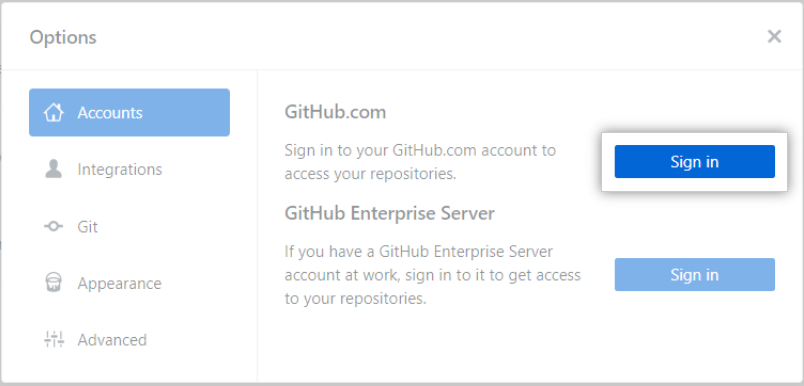
\includegraphics[width=0.3\textwidth]{figures/Account Options.png}
    \caption{Account Options}
\end{figure}


\subsubsection{Part 2: Configuring and customizing GitHub Desktop}
After you install GitHub Desktop, you can configure and customize the app to best suit your needs.
You can connect or remove accounts on GitHub or GitHub Enterprise, choose a default text editor or shell, edit your Git configuration, change the appearance of GitHub Desktop, customize system dialogs, and set privacy preferences in the GitHub Desktop Options window. For more information, see "Configuring basic settings".

\begin{figure}[ht]
    \centering
    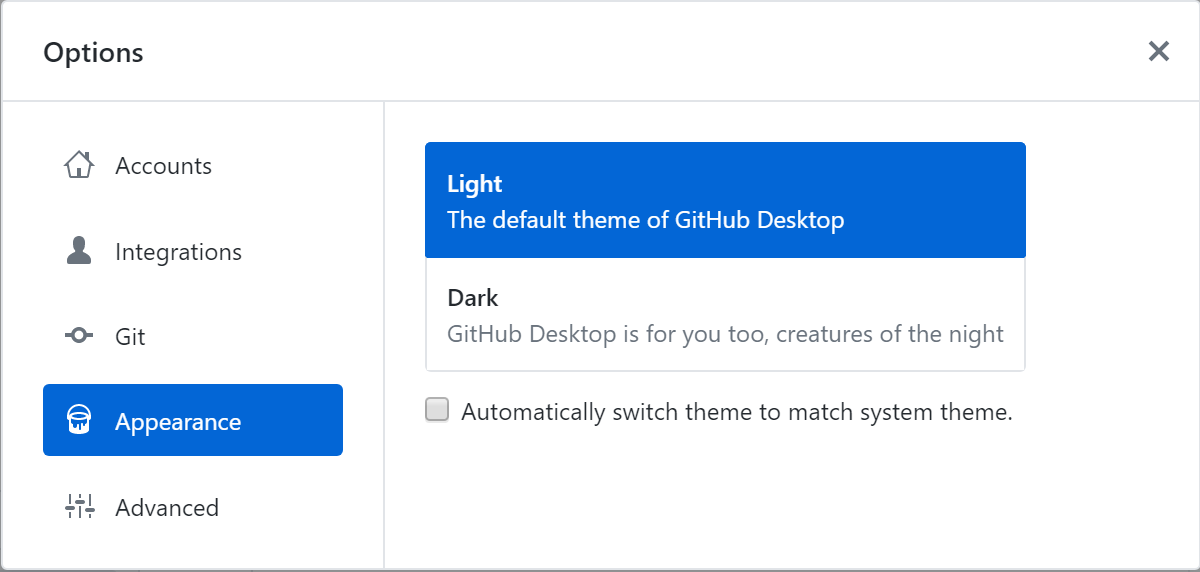
\includegraphics[width=0.3\textwidth]{figures/Appearance Options.png}
    \caption{Appearance Options}
\end{figure}


\subsubsection{Part 3: Contributing to projects with GitHub Desktop}

After installing, authenticating, and configuring the app, you are ready to start using GitHub Desktop. You can create, add, or clone repositories and use GitHub Desktop to manage contributions to your repositories.
Creating, adding, and cloning repositories
You can create a new repository by selecting the File menu and clicking New repository.... For more information, see "Creating your first repository using GitHub Desktop."
You can add a repository from your local computer by selecting the File menu and clicking Add Local Repository.... For more information, see "Adding a repository from your local computer to GitHub Desktop."
You can clone a repository from GitHub by selecting the File menu and clicking Clone Repository.... For more information, see "Cloning and Forking Repositories from GitHub Desktop."

\begin{figure}[ht]
    \centering
    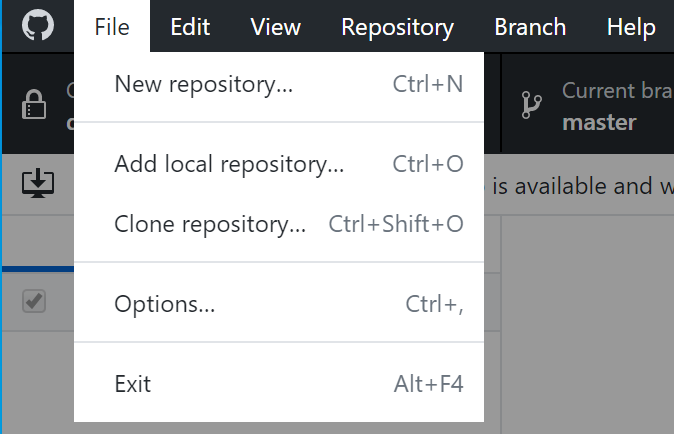
\includegraphics[width=0.3\textwidth]{figures/Cloning and Forking Repositories from GitHub Desktop.png}
    \caption{Cloning and Forking Repositories }
\end{figure}

Making changes in a branch
You can use GitHub Desktop to create a branch of a project. Branches isolate your development work from other branches in the repository, so that you can safely experiment with changes. For more information, see "Managing branches."
 
After you make changes to a branch, you can review them in GitHub Desktop and make a commit to keep track of your changes. For more information, see "Committing and reviewing changes to your project."

\begin{figure}[ht]
    \centering
    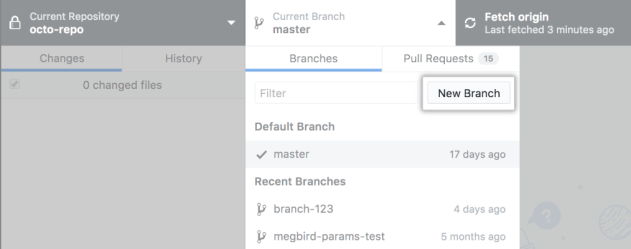
\includegraphics[width=0.3\textwidth]{figures/Managing branches.png}
    \caption{Managing branches}
\end{figure}









\subsection{ Creating your first repository using GitHub Desktop }
You can use GitHub Desktop to create and manage a Git repository without using the command line.

\subsubsection{ Introduction}
GitHub Desktop extends and simplifies your GitHub.com workflow, using a visual interface instead of text commands on the command line. By the end of this guide, you'll have used GitHub Desktop to create a repository, make changes to the repository, and publish the changes to GitHub.
After installing GitHub Desktop and signing into GitHub or GitHub Enterprise you can create and clone a tutorial repository. The tutorial will introduce the basics of working with Git and GitHub, including installing a text editor, creating a branch, making a commit, pushing to GitHub.com, and opening a pull request. The tutorial is available if you do not have any repositories on GitHub Desktop yet.
We recommend completing the tutorial, but if you want to explore GitHub Desktop by creating a new repository, this guide will walk you through using GitHub Desktop to work on a Git repository.

\subsubsection{Part 1: Installing GitHub Desktop and authenticating your account}

You can install GitHub Desktop on any supported operating system. After you install the app, you will need to sign in and authenticate your account on GitHub or GitHub Enterprise before you can create and clone a tutorial repository.
For more information on installing and authenticating, see "Setting up GitHub Desktop."

\subsubsection{Part 2: Creating a new repository}

If you do not have any repositories associated with GitHub Desktop, you will see a "Let's get started!" view, where you can choose to create and clone a tutorial repository, clone an existing repository from the Internet, create a new repository, or add an existing repository from your hard drive.

\begin{figure}[ht]
    \centering
    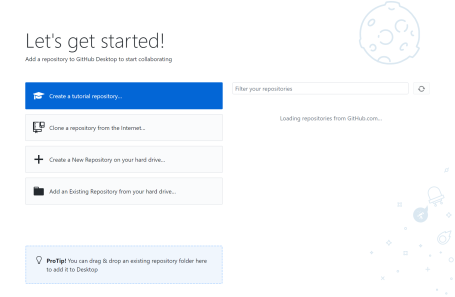
\includegraphics[width=0.3\textwidth]{figures/Setting up GitHub Desktop.png}
    \caption{Setting up GitHub Desktop}
\end{figure}

Creating and cloning a tutorial repository:
We recommend that you create and clone a tutorial repository as your first project to practice using GitHub Desktop.

1.Click Create a tutorial repository and clone it.
\begin{figure}[ht]
    \centering
    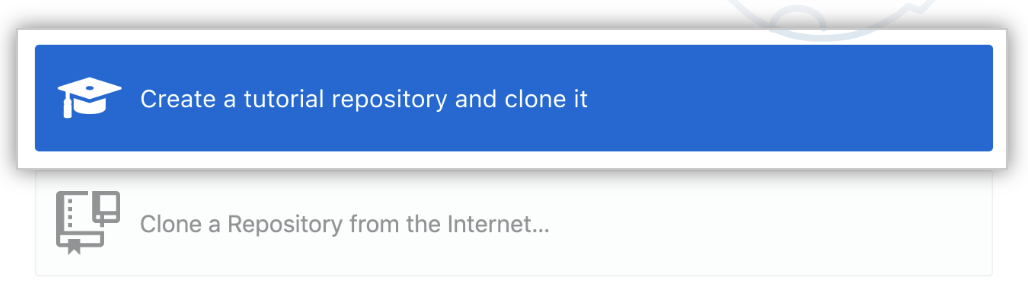
\includegraphics[width=0.3\textwidth]{figures/Creating a tutorial repository and clone it.png}
    \caption{Creating a tutorial repository and clone it}
\end{figure}

2.Follow the prompts in the tutorial to install a text editor, create a branch, edit a file, make a commit, publish to GitHub, and open a pull request.





Creating a new repository:
If you do not wish to create and clone a tutorial repository, you can create a new repository.

1.Click Create a New Repository on your Hard Drive....

\begin{figure}[ht]
    \centering
    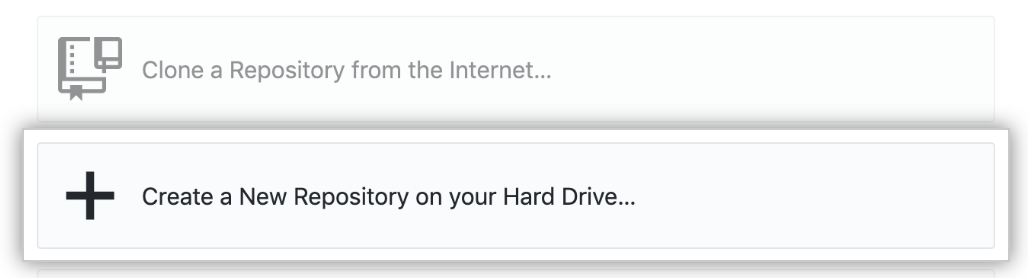
\includegraphics[width=0.3\textwidth]{figures/Creating a New Repository on your Hard Drive.png}
    \caption{Creating a New Repository on your Hard Drive}
\end{figure}


2.Fill in the fields and select your preferred options.
\begin{figure}[ht]
    \centering
    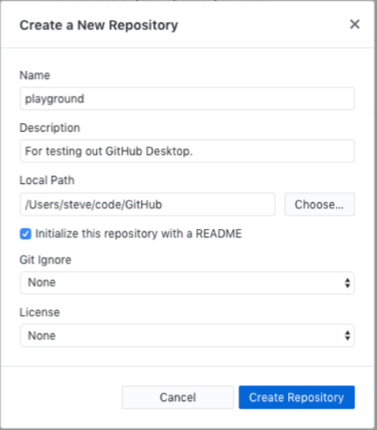
\includegraphics[width=0.3\textwidth]{figures/Creating a New Repository Window.png}
    \caption{Creating a New Repository Window}
\end{figure}





\subsubsection{Part 3: Exploring GitHub Desktop}

In the file menu at the top of the screen, you can access settings and actions that you can perform in GitHub Desktop. Most actions also have keyboard shortcuts to help you work more efficiently. For a full list of keyboard shortcuts, see "Keyboard shortcuts."


The GitHub Desktop menu bar :
At the top of the GitHub Desktop app, you will see a bar that shows the current state of your repository.

•	Current repository shows the name of the repository you're working on. You can click Current repository to switch to a different repository in GitHub Desktop.

•	Current branch shows the name of the branch you're working on. You can click Current branch to view all the branches in your repository, switch to a different branch, or create a new branch. Once you create pull requests in your repository, you can also view these by clicking on Current branch.

•	Publish repository appears because you haven't published your repository to GitHub yet, which you'll do later in the next step. This section of the bar will change based on the status of your current branch and repository. Different context dependent actions will be available that let you exchange data between your local and remote repositories.
\begin{figure}[ht]
    \centering
    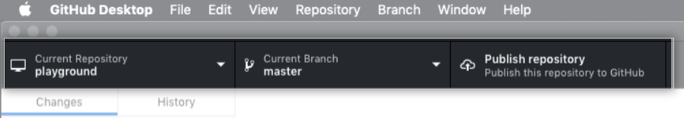
\includegraphics[width=0.3\textwidth]{figures/The GitHub Desktop menu bar.png}
    \caption{The GitHub Desktop menu bar}
\end{figure}


Changes and History
In the left sidebar, you'll find the Changes and History views. 

\begin{figure}[ht]
    \centering
    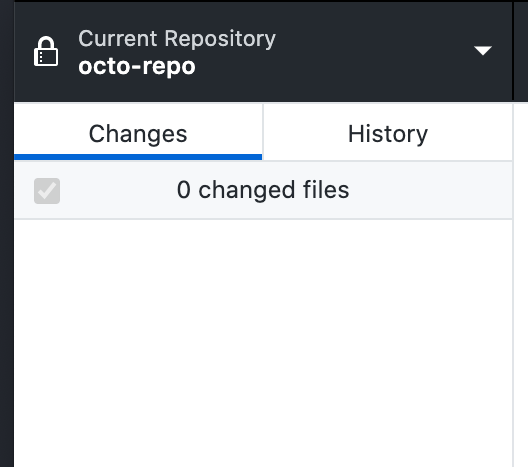
\includegraphics[width=0.3\textwidth]{figures/the Changes and History views.png}
    \caption{the Changes and History views}
\end{figure}


•	The Changes view shows changes you've made to files in your current branch but haven't committed to your local repository. At the bottom, there is a box with "Summary" and "Description" text boxes and a Commit to BRANCH button. This is where you'll commit new changes. The Commit to BRANCH button is dynamic and will display which branch you're committing your changes to.  
\begin{figure}[ht]
    \centering
    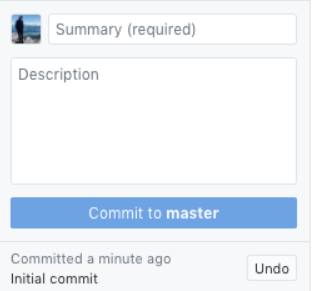
\includegraphics[width=0.3\textwidth]{figures/Commit to BRANCH.png}
    \caption{Commit to BRANCH}
\end{figure}

•	The History view shows the previous commits on the current branch of your repository. You should see an "Initial commit" that was created by GitHub Desktop when you created your repository. To the right of the commit, depending on the options you selected while creating your repository, you may see .git attributes, .gitignore, LICENSE, or README files. You can click each file to see a diff for that file, which is the changes made to the file in that commit. The diff only shows the parts of the file that have changed, not the entire contents of the file. 
\begin{figure}[ht]
    \centering
    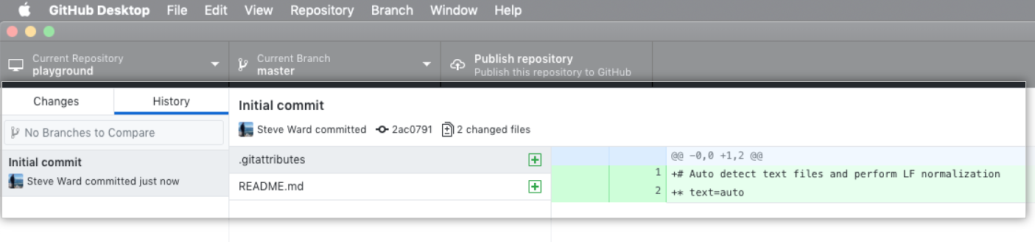
\includegraphics[width=0.3\textwidth]{figures/The History view.png}
    \caption{The History view}
\end{figure}



\subsubsection{Part 4: Publishing your repository to GitHub}

When you create a new repository, it only exists on your computer and you are the only one who can access the repository. You can publish your repository to GitHub to keep it synchronized across multiple computers and allow other people to access it. To publish your repository, push your local changes to GitHub.

1.	Click Publish repository in the menu bar.
\begin{figure}[ht]
    \centering
    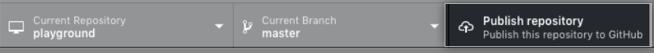
\includegraphics[width=0.3\textwidth]{figures/The menu bar.png}
    \caption{The menu bar}
\end{figure}
 
o	GitHub Desktop automatically fills the "Name" and "Description" fields with the information you entered when you created the repository.
o	Keep this code private lets you control who can view your project. If you leave this option unselected, other users on GitHub will be able to view your code. If you select this option, your code will not be publicly available.
o	The Organization drop-down menu, if present, lets you publish your repository to a specific organization that you belong to on GitHub.
\begin{figure}[ht]
    \centering
    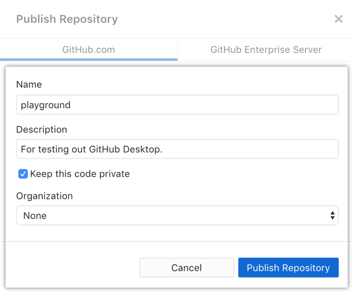
\includegraphics[width=0.3\textwidth]{figures/Publish repository window.png}
    \caption{Publish repository window}
\end{figure}


2.	Click the Publish Repository button.


3.	You can access the repository on GitHub.com from within GitHub Desktop. In the file menu, click Repository, then click View on GitHub. This will take you directly to the repository in your default browser.




\subsubsection{Part 5: Making, committing, and pushing changes}
Now that you've created and published your repository, you're ready to make changes to your project and start crafting your first commit to your repository.
1.	To launch your external editor from within GitHub Desktop, click Repository, then click Open in EDITOR. For more information, see "Configuring a default editor."
\begin{figure}[ht]
    \centering
    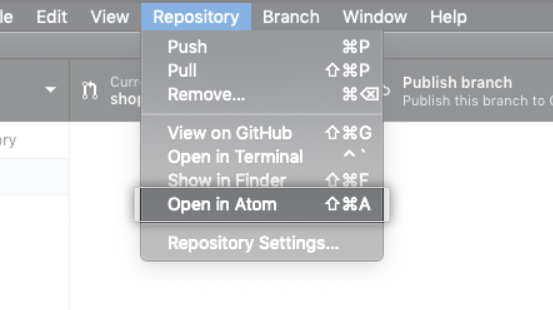
\includegraphics[width=0.3\textwidth]{figures/Open in EDITOR.png}
    \caption{Open in EDITOR}
\end{figure}
 
2.	Make some changes to the README.md file that you previously created. You can add information that describes your project, like what it does and why it is useful. When you are satisfied with your changes, save them in your text editor.

3.	In GitHub Desktop, navigate to the Changes view. In the file list, you should see your README.md. The checkmark to the left of the README.md file indicates that the changes you've made to the file will be part of the commit you make. In the future, you might make changes to multiple files but only want to commit the changes you've made to some of the files. If you click the checkmark next to a file, that file will not be included in the commit.
\begin{figure}[ht]
    \centering
    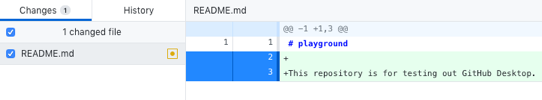
\includegraphics[width=0.3\textwidth]{figures/The Changes view.png}
    \caption{The Changes view}
\end{figure}
 
4.	At the bottom of the Changes list, enter a commit message. To the right of your profile picture, type a short description of the commit. Since we're changing the README.md file, "Add information about purpose of project" would be a good commit summary. Below the summary, you'll see a "Description" text field where you can type a longer description of the changes in the commit, which is helpful when looking back at the history of a project and understanding why changes were made. Since you're making a basic update of a README.md file, you can skip the description.
\begin{figure}[ht]
    \centering
    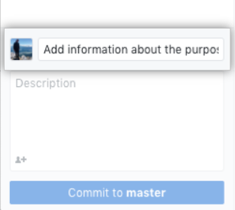
\includegraphics[width=0.3\textwidth]{figures/The Changes list.png}
    \caption{The Changes list}
\end{figure}

5.	Click Commit to BRANCH NAME. The commit button shows your current branch so you can be sure to commit to the branch you want.
\begin{figure}[ht]
    \centering
    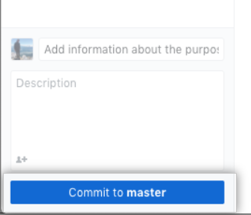
\includegraphics[width=0.3\textwidth]{figures/Commit to BRANCH NAME.png}
    \caption{Commit to BRANCH NAME}
\end{figure}
6.	Click Commit to master. The commit button shows your current branch, which in this case is master, so that you know which branch you are making a commit to.

\begin{figure}[ht]
    \centering
    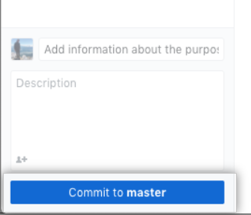
\includegraphics[width=0.3\textwidth]{figures/Commit to master.png}
    \caption{Commit to master}
\end{figure}


7.	To push your changes to the remote repository on GitHub, click Push origin.

\begin{figure}[ht]
    \centering
    
\includegraphics[width=0.3\textwidth]{figures/Push origin.png}
    \caption{Push origin}
\end{figure}


•	The Push origin button is the same one that you clicked to publish your repository to GitHub. This button changes contextually based on where you are at in the Git workflow. It should now say Push origin with a 1 next to it, indicating that there is one commit that has not been pushed up to GitHub.
•	The "origin" in Push origin means that you are pushing changes to the remote called origin, which in this case is your project's repository on GitHub.com. Until you push any new commits to GitHub, there will be differences between your project's repository on your computer and your project's repository on GitHub.com. This allows you to work locally and only push your changes to GitHub.com when you're ready.

1.	In the window to the right of the Changes view, you'll see suggestions for actions you can do next. To open the repository on GitHub in your browser, click View on GitHub.
\begin{figure}[ht]
    \centering
    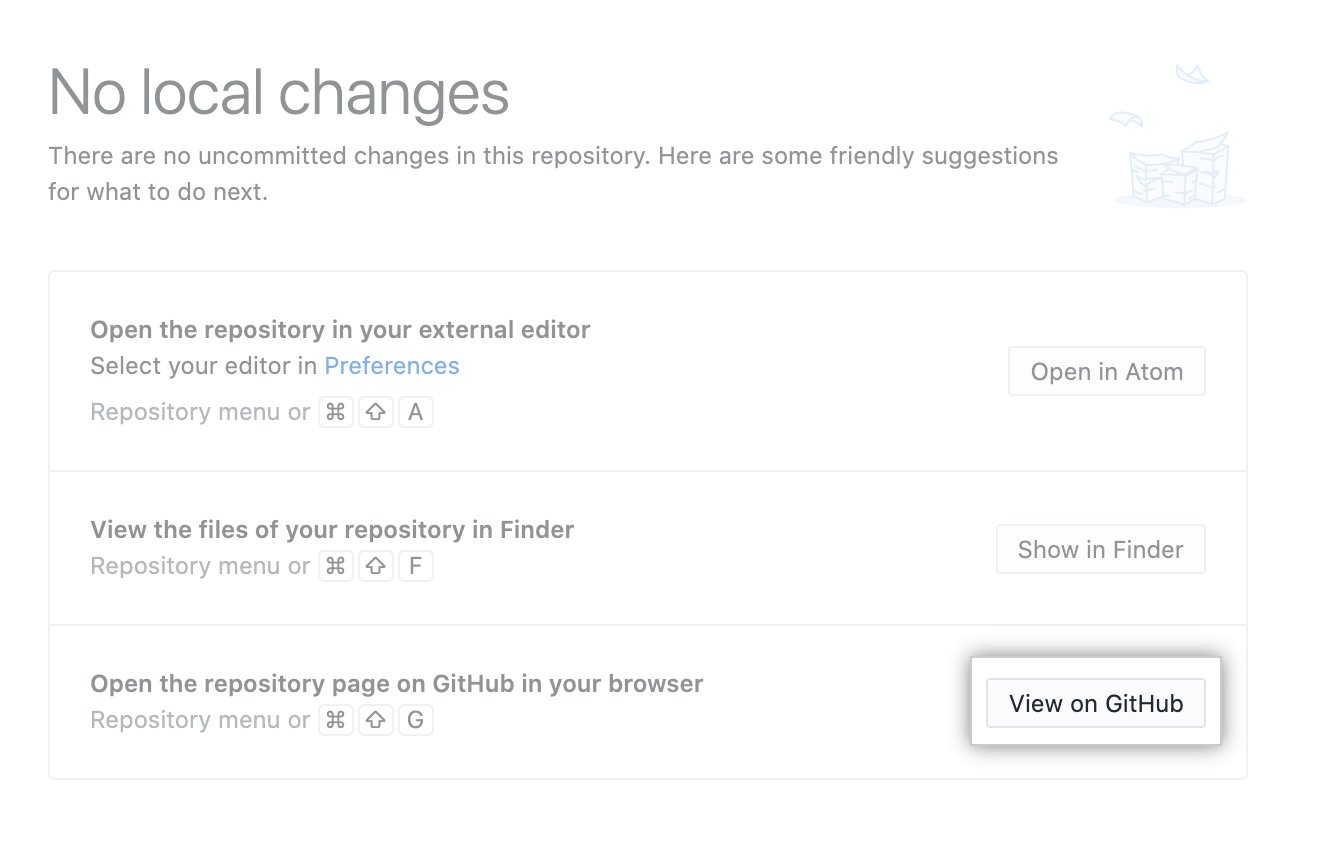
\includegraphics[width=0.3\textwidth]{figures/Changes view.png}
    \caption{Changes view}
\end{figure}
 
2.	In your browser, click 2 commits. You'll see a list of the commits in this repository on GitHub. The first commit should be the commit you just made in GitHub Desktop.
\begin{figure}[ht]
    \centering
    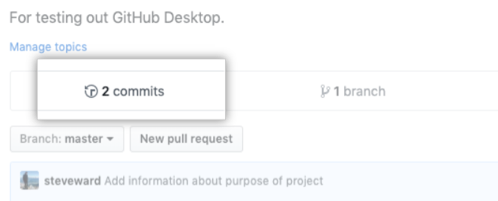
\includegraphics[width=0.3\textwidth]{figures/2 commits.png}
    \caption{2 commits}
\end{figure}

 
Conclusion
You've now created a repository, published the repository to GitHub, made a commit, and pushed your changes to GitHub. You can follow this same workflow when contributing to other projects that you create or collaborate on.

\subsection{ Supported operating systems}
You can use GitHub Desktop on any supported operating system.


\subsubsection{About supported operating systems}

The following operating systems are supported for GitHub Desktop.

•	macOS 10.10 or later
•	Windows 7 64-bit or later. You must have a 64-bit operating system to run GitHub Desktop.


\subsubsection{- Troubleshooting problems on macOS}

If you're encountering problems using GitHub Desktop on macOS, here are resolutions to try. For more information, see known-issues.
The username or passphrase you entered is not correct error after signing into your account
This error can occur when GitHub Desktop can't access your stored credentials on Keychain.
To troubleshoot this error, follow these steps.

1.	Open the "Keychain Access" app.


2.	Right-click on login and then click Lock Keychain "login".

\begin{figure}[ht]
    \centering
    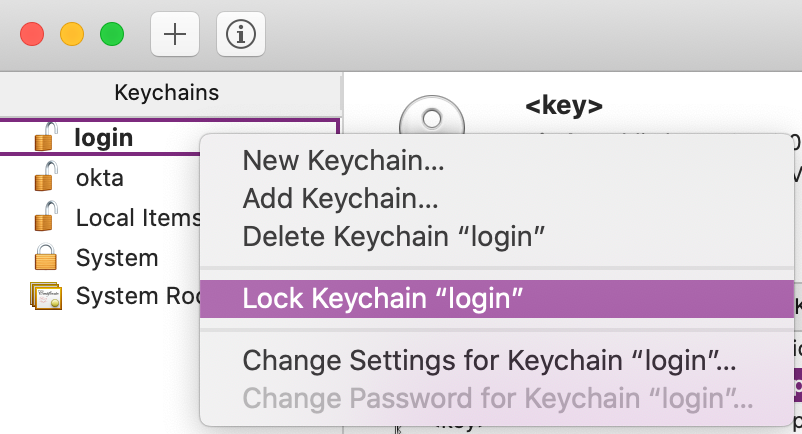
\includegraphics[width=0.3\textwidth]{figures/Lock Keychain.png}
    \caption{Lock Keychain}
\end{figure}
 
 
3.	Right-click on login and then click Unlock Keychain "login". Follow any onscreen prompts to finish unlocking the Keychain "login."

\begin{figure}[ht]
    \centering
    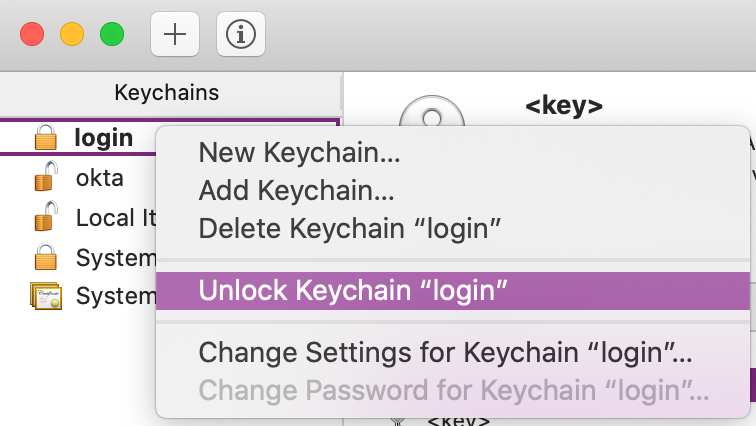
\includegraphics[width=0.3\textwidth]{figures/Unlock Keychain.png}
    \caption{Unlock Keychain}
\end{figure}
 
 
4.	Re-authenticate your account on GitHub or GitHub Enterprise.
Could not create temporary directory: Permission denied error after checking for updates
This error can be caused by missing permissions for the ~/Library/Caches/com.github.GitHubClient.ShipIt directory. GitHub Desktop uses this directory to create and unpack temporary files as part of updating the application.
To troubleshoot this error, follow these steps.
1.	Close GitHub Desktop.
2.	Open "Finder" and navigate to ~/Library/Caches/.
3.	Right-click com.github.GitHubClient.ShipIt and then click Get Info.
4.	Click the arrow to the left of "Sharing and Permissions."

5.	If the Privilege to the right of your user account does not say "Read and Write," click the text and then click Read and Write.
\begin{figure}[ht]
    \centering
    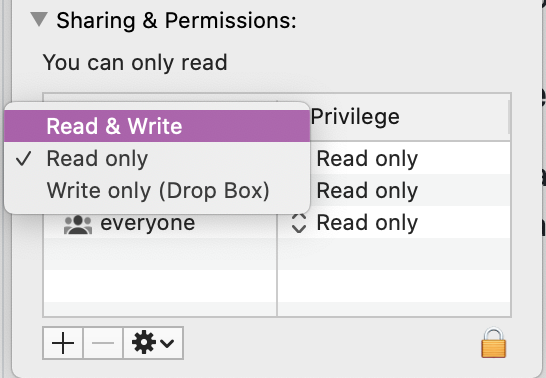
\includegraphics[width=0.3\textwidth]{figures/Read & Write.png}
    \caption{Read and Write}
\end{figure}

6.	Open GitHub Desktop and check for updates.

\subsubsection{- Troubleshooting problems on Windows}

If you're encountering problems using GitHub Desktop on Windows, here are resolutions to try. For more information, see known-issues.

The revocation function was unable to check revocation for the certificate. error
This error can occur if you are using GitHub Desktop on a corporate network that blocks Windows from checking the revocation status of a certificate.

To troubleshoot, contact your system administrator.

git clone failed error while cloning a repository configured with Folder Redirection
GitHub Desktop does not support repositories configured with Folder Redirection.
cygheap base mismatch detected error
This error can occur when Mandatory ASLR is enabled. Enabling Mandatory ASLR affects the MSYS2 core library, which GitHub Desktop relies upon to emulate process forking.

To troubleshoot this error, either disable Mandatory ASLR or explicitly allow all executables under

<Git>\ usr\ bin which depend on MSYS2.



\subsection{ Launching GitHub Desktop from the command line}

You can launch GitHub Desktop from the command line.

\subsubsection{- For Windows }

1.	Open a command prompt.
2.	To launch GitHub Desktop to the last opened repository, type github. To launch GitHub Desktop for a particular repository, type github followed by the path to the repository.
C:\ Users\ octocat> github path\ to\ repo
You can also change to your repository path and then type github . to open that repository.
C:\ Users\ octocat> cd repo\ myrepo
 C:\ Users\ octocat\ repo\ myrepo> github .
  
 \subsubsection{- For Mac }
1.	In the menu bar, select the GitHub Desktop menu, then click Install Command Line Tool.

\begin{figure}[ht]
    \centering
    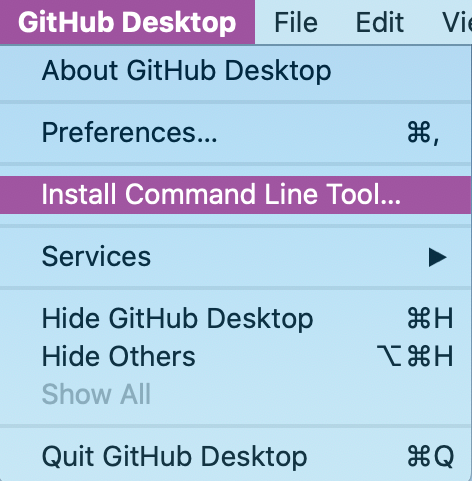
\includegraphics[width=0.3\textwidth]{figures/Install Command Line Tool.png}
    \caption{Install Command Line Tool}
\end{figure}


2.	Open Terminal.
3.	To launch GitHub Desktop to the last opened repository, type github. To launch GitHub Desktop for a particular repository, type github followed by the path to the repository.
$ github / path / to/ repo $
You can also change to your repository path and then type github .
to open that repository.
$ cd /path/to/repo $
[repo] $  github .$



 \subsection{Installing and authenticating to GitHub Desktop }
 
\textbf{Setting up GitHub Desktop }

You can set up GitHub Desktop to suit your needs and contribute to projects.

\subsubsection{Part 1: Installing GitHub Desktop}
You can install GitHub Desktop on any supported operating system. For more information, see "Supported Operating Systems."
To install GitHub Desktop, navigate to https://desktop.github.com/ and download the appropriate version of GitHub Desktop for your operating system. Follow the prompts to complete the installation. For more information, see "Installing GitHub Desktop."

\subsubsection{Part 2: Configuring your account}

If you have an account on GitHub or GitHub Enterprise, you can use GitHub Desktop to exchange data between your local and remote repositories.
Creating an account
If you do not already have an account on GitHub, see "Signing up for a new GitHub account."
If you are part of an organization that uses GitHub Enterprise and you do not have an account, contact your GitHub Enterprise site administrator.
Authenticating to GitHub
To connect to GitHub Desktop with GitHub, you'll need to authenticate your account. For more information, see "Authenticating to GitHub Desktop."
After authenticating your account, you are ready to manage and contribute to projects with GitHub Desktop.

\subsubsection{Part 3: Configuring Git }

You must have Git installed before using GitHub Desktop. If you do not already have Git installed, you can download and install the latest version of Git from https://git-scm.com/downloads.
After you have Git installed, you'll need to configure Git for GitHub Desktop. For more information, see "Configuring Git for GitHub Desktop."

\subsubsection{Part 4: Customizing GitHub Desktop }
You can adjust defaults and settings to tailor GitHub Desktop to your needs.
- Choosing a default text editor
You can open a text editor from GitHub Desktop to manipulate files and repositories. GitHub Desktop supports a variety of text editors and integrated development environments (IDEs) for Windows and macOS. You can choose a default editor in the GitHub Desktop settings. For more information, see "Configuring a default editor."

- Choosing a theme
GitHub Desktop has multiple themes available to customize the look and feel of the app. You can choose a theme in the GitHub Desktop settings. For more information, see "Setting a theme for GitHub Desktop."





\subsection{Installing GitHub Desktop }

You can install GitHub Desktop on supported Windows or macOS operating systems.

\subsubsection{- For Windows }

About GitHub Desktop installation: 

You can install GitHub Desktop on supported operating systems. If you have an account on GitHub or GitHub Enterprise, you can connect your account to GitHub Desktop. For more information about creating an account, see "Signing up for a new GitHub account" or contact your GitHub Enterprise site administrator.

If you are a network administrator, you can deploy GitHub Desktop to computers running Windows on an Active Directory-managed network by using the Windows Installer package file (.msi) with Group Policy or another remote installation system.

The Windows Installer package extracts the standalone installer (.exe) and configures Windows to install GitHub Desktop the next time a user signs in to their workstation. Users must have permissions to install GitHub Desktop in their user directory.

If a user runs the Windows Installer package for GitHub Desktop directly, to complete the installation, the user must sign out of their workstation and then sign back in.

Downloading and installing GitHub Desktop
You can install GitHub Desktop on Windows 7 64-bit or later.

Warning: You must have a 64-bit operating system to run GitHub Desktop.
1.	Visit the download page for GitHub Desktop.
2.	Click Download for Windows.
\begin{figure}[ht]
    \centering
    
\includegraphics[width=0.3\textwidth]{figures/Download for Windows.png}
    \caption{Download for Windows}
\end{figure}

3. In your computer's Downloads folder, double-click the GitHub Desktop setup file.
\begin{figure}[ht]
    \centering
    
\includegraphics[width=0.3\textwidth]{figures/the GitHub Desktop setup file.png}
    \caption{the GitHub Desktop setup file}
\end{figure}

4. GitHub Desktop will launch after installation is complete.



\subsubsection{- For Mac}

About GitHub Desktop installation:

You can install GitHub Desktop on supported operating systems. If you have an account on GitHub or GitHub Enterprise, you can connect your account to GitHub Desktop. For more information about creating an account, see "Signing up for a new GitHub account" or contact your GitHub Enterprise site administrator.

Downloading and installing GitHub Desktop
You can install GitHub Desktop on macOS 10.10 or later.
1.	Visit the download page for GitHub Desktop.
2.	Click Download for macOS.
\begin{figure}[ht]
    \centering
    
\includegraphics[width=0.3\textwidth]{figures/Download for macOS.png}
    \caption{Download for macOS}
\end{figure}

3.	In your computer's Downloads folder, double-click the GitHub Desktop zip file.
\begin{figure}[ht]
    \centering
    
\includegraphics[width=0.3\textwidth]{figures/the GitHub Desktop zip file.png}
    \caption{the GitHub Desktop zip file}
\end{figure}

4.	After the file has been unzipped, double-click GitHub Desktop.
5.	GitHub Desktop will launch after installation is complete.



\subsection{Authenticating to GitHub }

You can securely access your account's resources on GitHub Desktop by authenticating to GitHub.

\subsubsection{- For Windows }

About authentication:

To keep your account secure, you must authenticate before you can use GitHub Desktop to access resources on GitHub.

Before you authenticate, you must already have a GitHub or GitHub Enterprise account.
•	For more information on creating a GitHub account, see "Signing up for a new GitHub account".
•	For a GitHub Enterprise account, contact your GitHub Enterprise site administrator.

Authenticating an account on GitHub
1.	Use the File menu, then click Options.
\begin{figure}[ht]
    \centering
    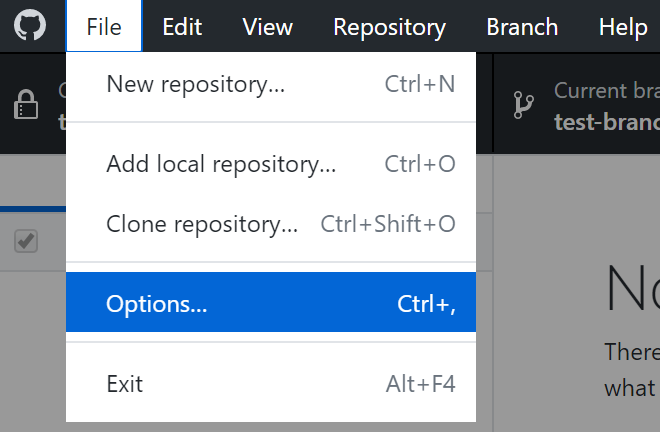
\includegraphics[width=0.3\textwidth]{figures/WIN Options.png}
    \caption{Windows Options }
\end{figure}
2.	In the Options window, select Accounts.
\begin{figure}[ht]
    \centering
    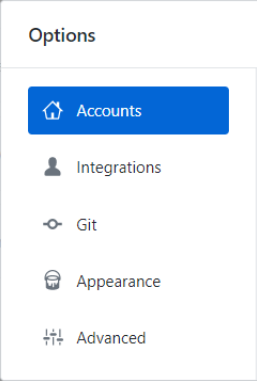
\includegraphics[width=0.3\textwidth]{figures/WIN Accounts.png}
    \caption{Windows Accounts}
\end{figure}
3.	To the right of "GitHub.com," click Sign in.
\begin{figure}[ht]
    \centering
    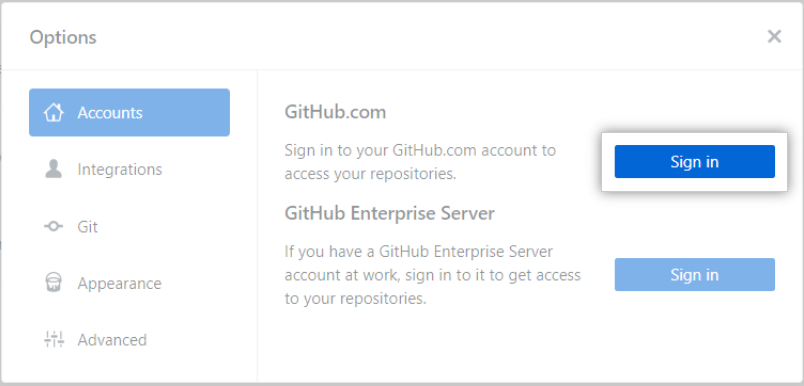
\includegraphics[width=0.3\textwidth]{figures/WIN Sign in.png}
    \caption{Windows sign in}
\end{figure}
4.	In the Sign in pane, click Sign in using your browser.
\begin{figure}[ht]
    \centering
    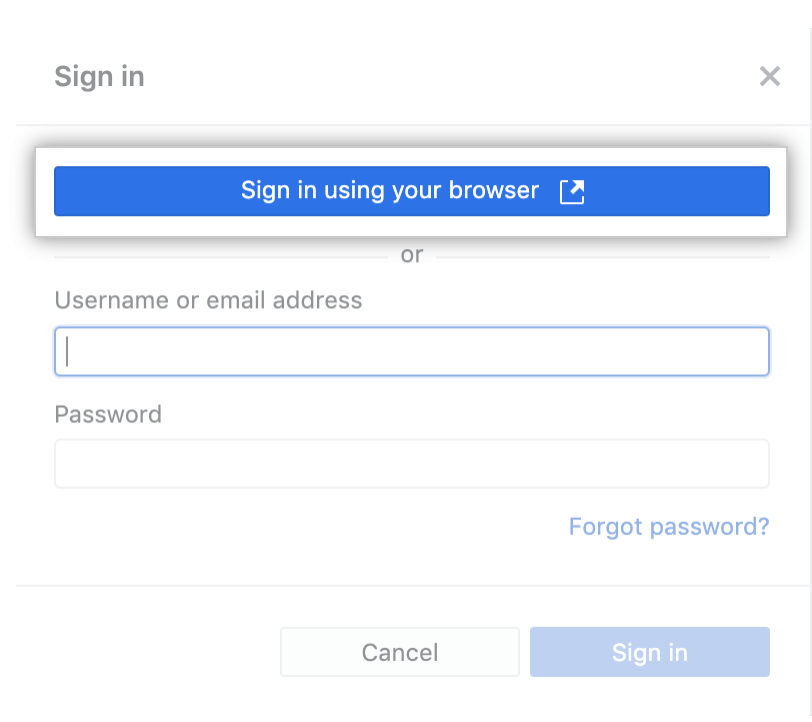
\includegraphics[width=0.3\textwidth]{figures/WIN Sign in using your browser.png}
    \caption{Windows Sign in using your browser}
\end{figure}
Warning: Authenticating to GitHub using your username and password is deprecated. We recommend authenticating using the browser instead.
5.	To authenticate to GitHub, type your GitHub.com credentials and click Sign in.
 
Alternatively, if you were already signed in to GitHub, follow the prompts to return to GitHub Desktop to finish authenticating.
\begin{figure}[ht]
    \centering
    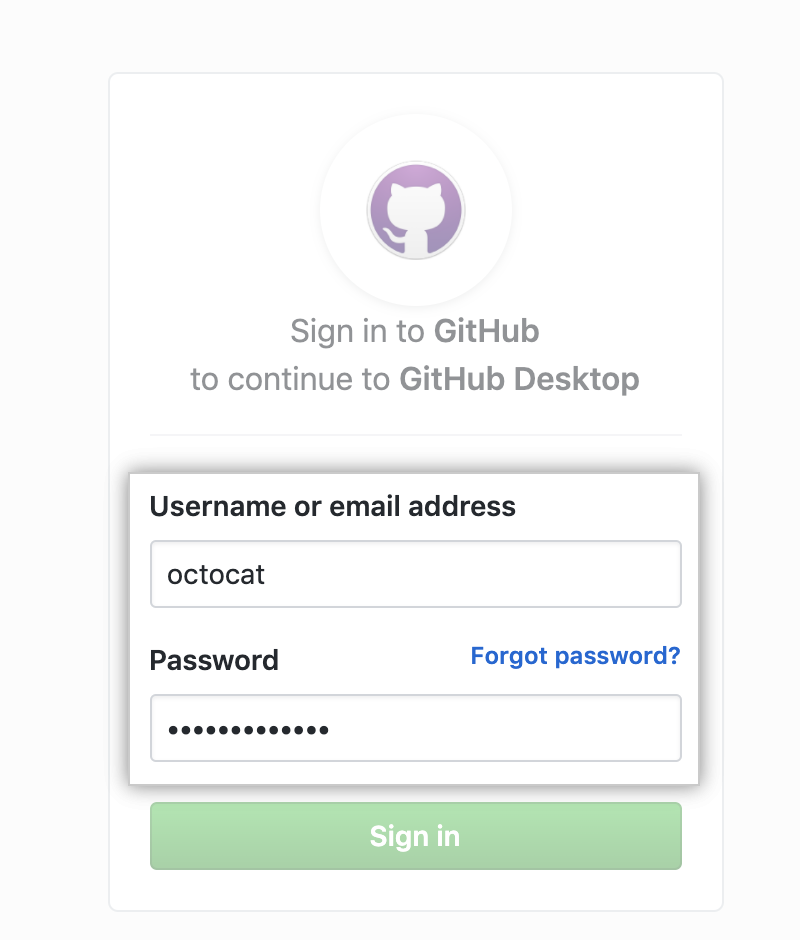
\includegraphics[width=0.3\textwidth]{figures/WIN click Sign in.png}
    \caption{Windows click Sign in }
\end{figure}
6.	If you have configured two-factor authentication (2FA) for GitHub, do one of the following:
o	If you set up 2FA via SMS, retrieve your 2FA code from an SMS message.
o	If you set up 2FA with a TOTP application, generate a 2FA code.

Then enter your 2FA code in the prompt on GitHub and click Verify.
 
\begin{figure}[ht]
    \centering
    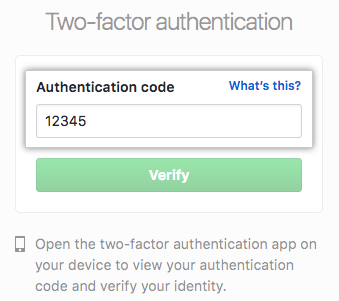
\includegraphics[width=0.3\textwidth]{figures/WIN Verify.png}
    \caption{WIN Verify}
\end{figure}


7.	After GitHub authenticates your account, follow the prompts to return to GitHub Desktop.
Authenticating an account on GitHub Enterprise
Warning: Authenticating to GitHub using your username and password is deprecated. We recommend authenticating using the browser instead.
1.	Use the File menu, then click Options.
\begin{figure}[ht]
    \centering
    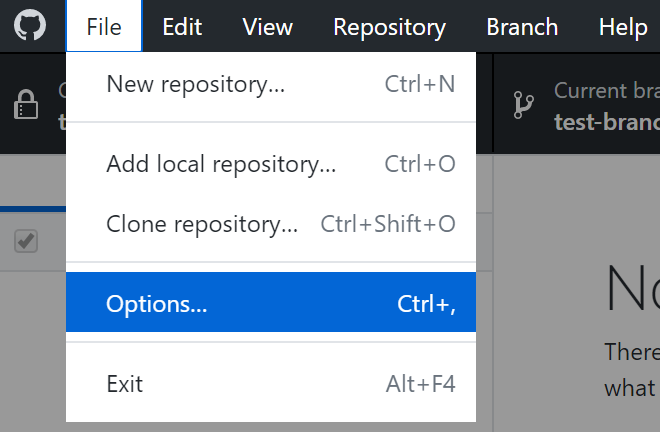
\includegraphics[width=0.3\textwidth]{figures/WIN EN Options.png}
    \caption{Windows enterprise Options}
\end{figure}
2.	In the Options window, select Accounts.
\begin{figure}[ht]
    \centering
    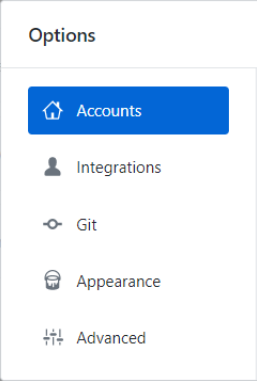
\includegraphics[width=0.3\textwidth]{figures/WIN EN Accounts.png}
    \caption{Windows enterprise accounts}
\end{figure}
3.	To the right of "GitHub Enterprise Server," click Sign In.
\begin{figure}[ht]
    \centering
    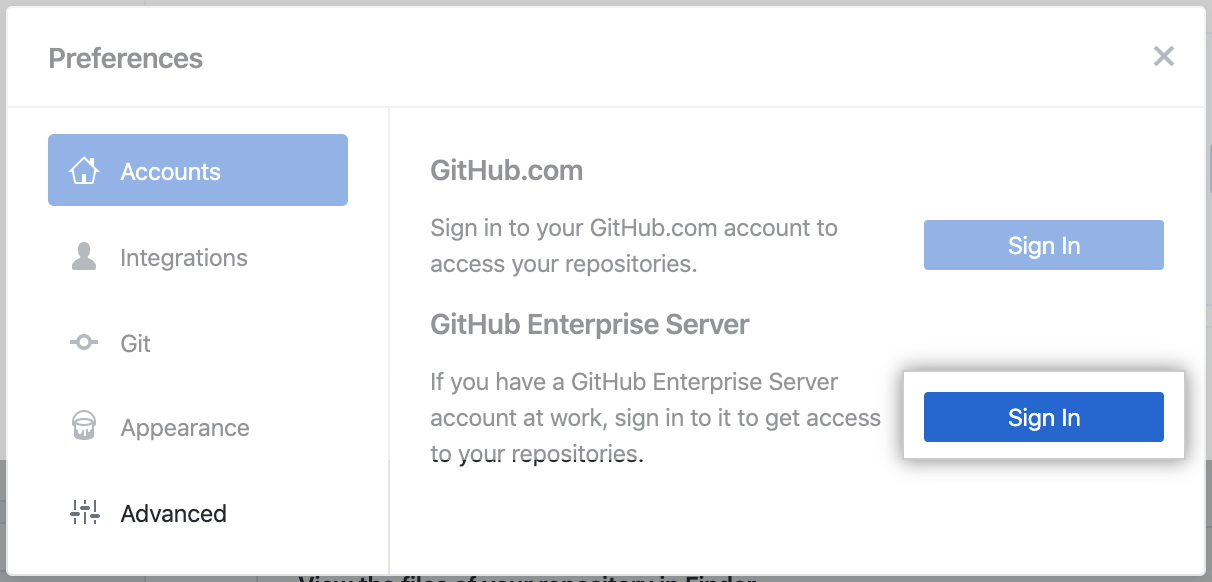
\includegraphics[width=0.3\textwidth]{figures/WIN EN Sign In.png}
    \caption{Windows enterprise sign in }
\end{figure}

4.	To add a GitHub Enterprise account, type your credentials under "Enterprise server address," then click Continue.
\begin{figure}[ht]
    \centering
    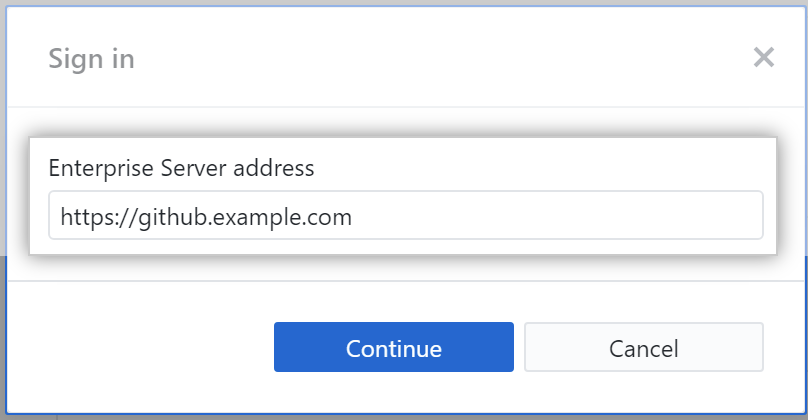
\includegraphics[width=0.3\textwidth]{figures/WIN EN Continue.png}
    \caption{Windows enterprise continue}
\end{figure}
5.	If you have configured two-factor authentication for GitHub Enterprise, do one of the following:
o	If you set up 2FA via SMS, retrieve your 2FA code from an SMS message.
o	If you set up 2FA with a TOTP application, generate a 2FA code.

Then enter your 2FA code in the prompt on GitHub Desktop and click Sign In.
\begin{figure}[ht]
    \centering
    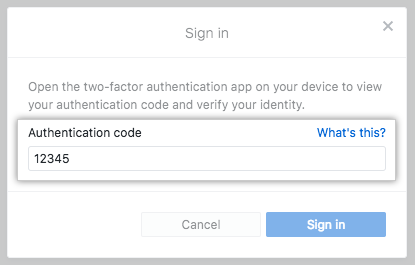
\includegraphics[width=0.3\textwidth]{figures/WIN EN click Sign In.png}
    \caption{Windows enterprise click sign in }
\end{figure}



\subsubsection{- For Mac }


About authentication:
To keep your account secure, you must authenticate before you can use GitHub Desktop to access resources on GitHub.

Before you authenticate, you must already have a GitHub or GitHub Enterprise account.

o For more information on creating a GitHub account, see "Signing up for a new GitHub account".
o For a GitHub Enterprise account, contact your GitHub Enterprise site administrator.


\textbf{Authenticating an account on GitHub}
1.	Use the File menu, then click Options.

\begin{figure}[ht]
    \centering
    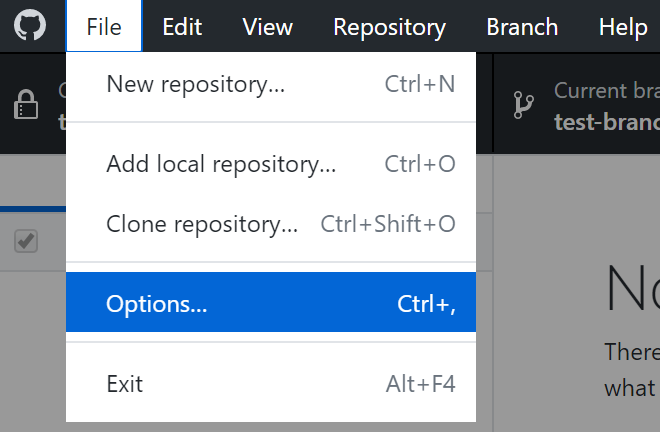
\includegraphics[width=0.3\textwidth]{figures/MAC Options.png}
    \caption{MAC Options}
\end{figure}

2.	In the Options window, select Accounts.

\begin{figure}[ht]
    \centering
    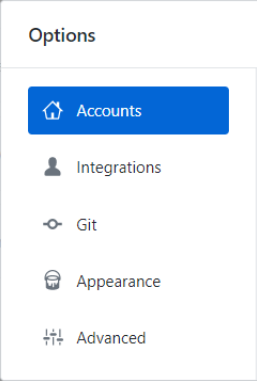
\includegraphics[width=0.3\textwidth]{figures/MAC Accounts.png}
    \caption{MAC Accounts}
\end{figure}

3.	To the right of "GitHub.com," click Sign in.
\begin{figure}[ht]
    \centering
    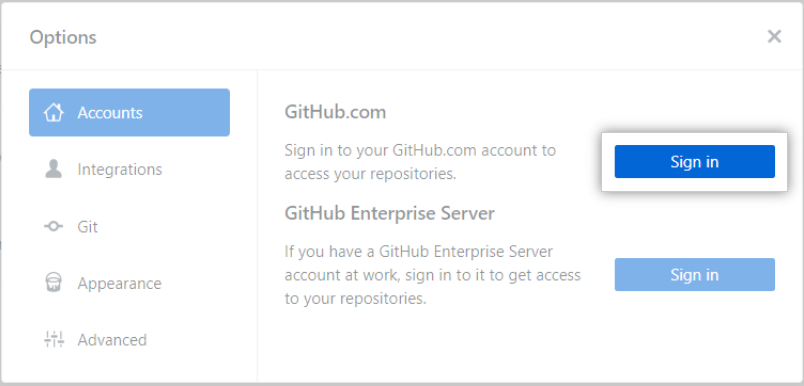
\includegraphics[width=0.3\textwidth]{figures/MAC Sign in.png}
    \caption{MAC Sign in}
\end{figure}


4.	In the Sign in pane, click Sign in using your browser. 

\begin{figure}[ht]
    \centering
    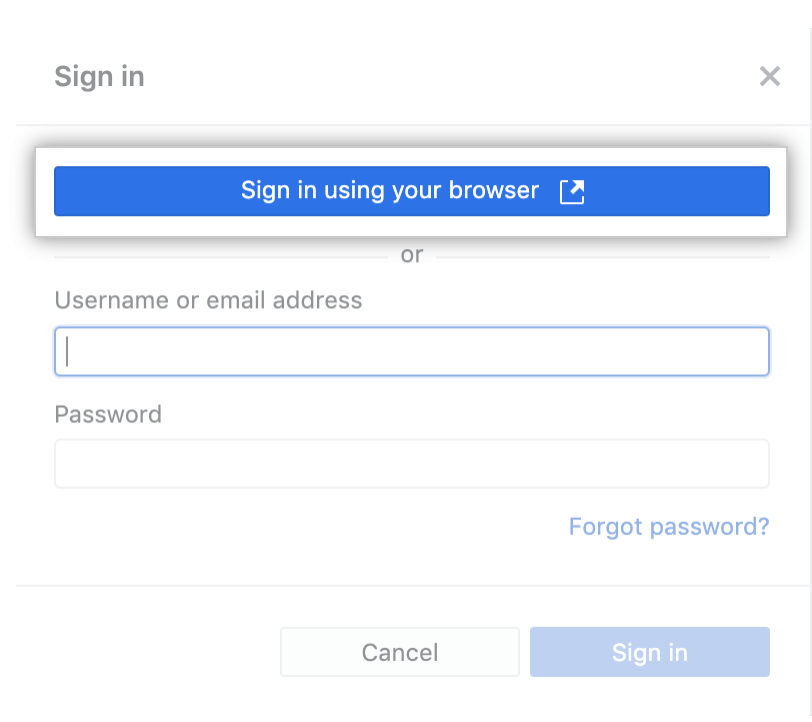
\includegraphics[width=0.3\textwidth]{figures/MAC Sign in using your browser.png}
    \caption{MAC Sign in using your browser}
\end{figure}

Warning: Authenticating to GitHub using your username and password is deprecated. We recommend authenticating using the browser instead.
5.	To authenticate to GitHub, type your GitHub.com credentials and click Sign in.

\begin{figure}[ht]
    \centering
    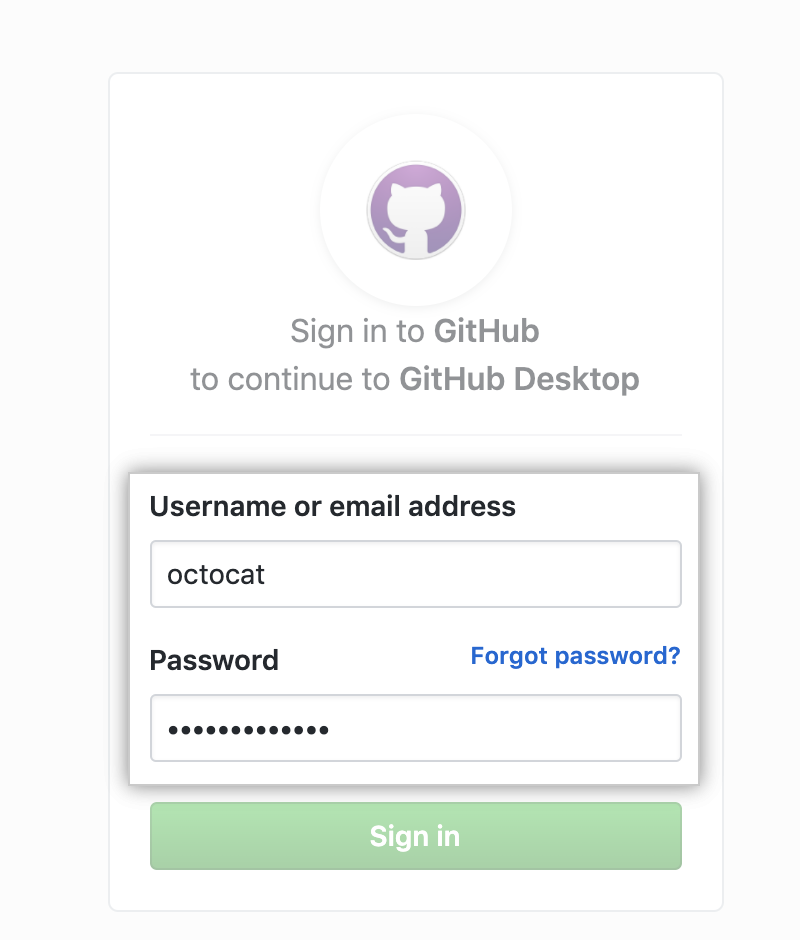
\includegraphics[width=0.3\textwidth]{figures/MAC click Sign in.png}
    \caption{MAC click Sign in}
\end{figure}

Alternatively, if you were already signed in to GitHub, follow the prompts to return to GitHub Desktop to finish authenticating.
6.	If you have configured two-factor authentication (2FA) for GitHub, do one of the following:
o	If you set up 2FA via SMS, retrieve your 2FA code from an SMS message.
o	If you set up 2FA with a TOTP application, generate a 2FA code.
Then enter your 2FA code in the prompt on GitHub and click Verify.
\begin{figure}[ht]
    \centering
    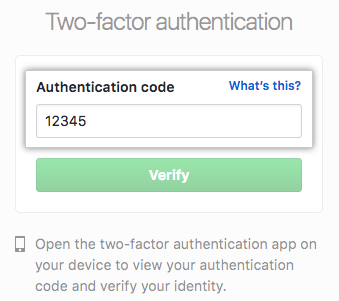
\includegraphics[width=0.3\textwidth]{figures/MAC Verify.png}
    \caption{MAC Verify}
\end{figure}

7.	After GitHub authenticates your account, follow the prompts to return to GitHub Desktop.
\textbf{Authenticating an account on GitHub Enterprise}
Warning: Authenticating to GitHub using your username and password is deprecated. We recommend authenticating using the browser instead.
1.	Use the File menu, then click Options.

\begin{figure}[ht]
    \centering
    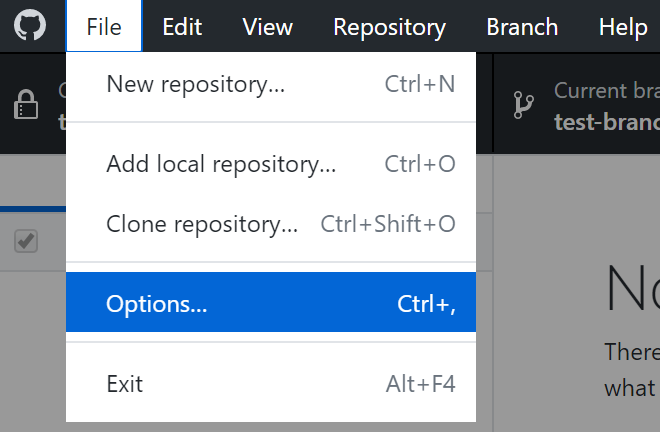
\includegraphics[width=0.3\textwidth]{figures/MAC EN Options.png}
    \caption{MAC Enterprise Options}
\end{figure}

2.	In the Options window, select Accounts.
\begin{figure}[ht]
    \centering
    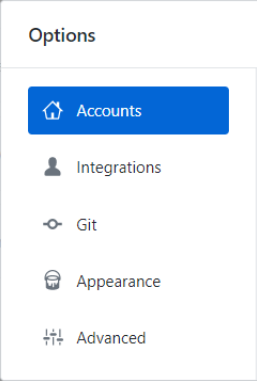
\includegraphics[width=0.3\textwidth]{figures/MAC EN Accounts.png}
    \caption{MAC Enterprise Accounts}
\end{figure}


3.	To the right of "GitHub Enterprise Server," click Sign In.
 \begin{figure}[ht]
    \centering
    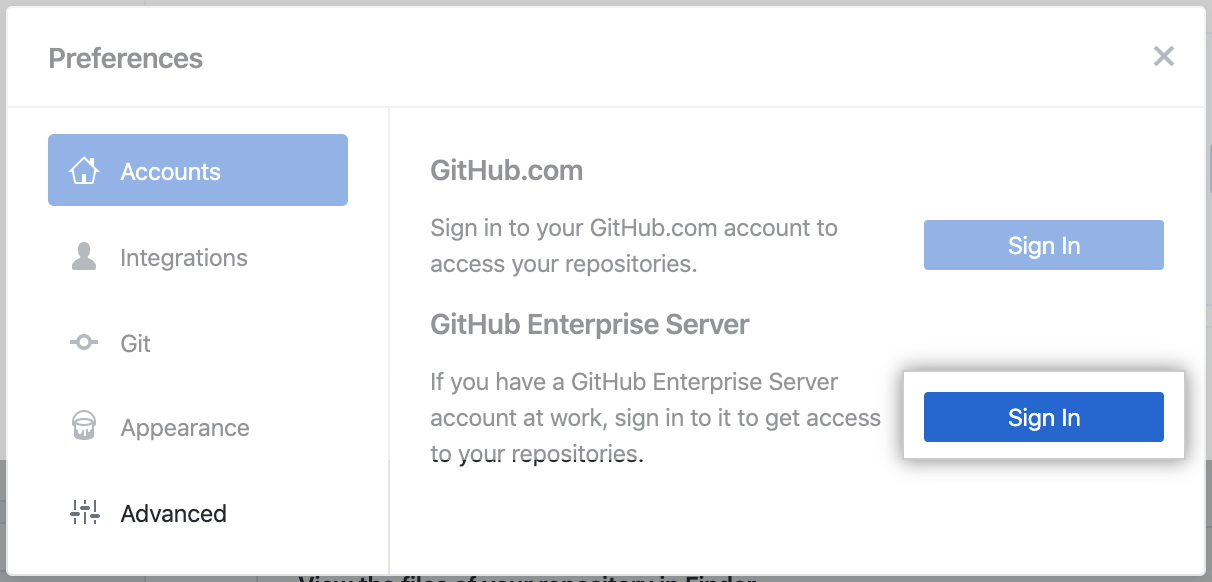
\includegraphics[width=0.3\textwidth]{figures/MAC EN Sign In.png}
    \caption{MAC Enterprise Sign In}
\end{figure}

4.	To add a GitHub Enterprise account, type your credentials under "Enterprise server address," then click Continue.

\begin{figure}[ht]
    \centering
    \includegraphics[width=0.3\textwidth]{figures/MAC EN Continue.png}
    \caption{MAC Enterprise Continue}
\end{figure}


5.	If you have configured two-factor authentication for GitHub Enterprise, do one of the following:
o	If you set up 2FA via SMS, retrieve your 2FA code from an SMS message.
o	If you set up 2FA with a TOTP application, generate a 2FA code.
Then enter your 2FA code in the prompt on GitHub Desktop and click Sign In.
 
\begin{figure}[ht]
    \centering
    \includegraphics[width=0.3\textwidth]{figures/MAC EN click Sign In.png}
    \caption{MAC Enterprise click Sign In}
\end{figure}

Troubleshooting authentication issues
If GitHub Desktop encounters an authentication error, you can use error messages to troubleshoot.
If you encounter an authentication error, first try signing out and signing back in to your account on GitHub Desktop.
For some errors, GitHub Desktop will prompt you with an error message. If you are not prompted, or to find more information about any error, view the GitHub Desktop log files by using the following steps.
1.	Use the Help drop-down menu and click Show Logs in Explorer.
\begin{figure}[ht]
    \centering
    \includegraphics[width=0.3\textwidth]{figures/Show Logs in Explorer.png}
    \caption{Show Logs in Explorer}
\end{figure}

2.	Select the log file from the date when you encountered the authentication error.
Review the troubleshooting information below for the error message that you encounter.

Bad credentials
Error: Bad credentials
This error means that there is an issue with your stored account credentials.

To troubleshoot, sign out of your account on GitHub Desktop and then sign back in.

Empty token
info: [ui] [AppStore.withAuthenticatingUser] account found for repository: node -  (empty token)
This error means that GitHub Desktop is unable to find the access token that it created in the system keychain.

To troubleshoot, sign out of your account on GitHub Desktop and then sign back in.

Repository not found
fatal: repository 'https://github.com//.git' not found

(The error was parsed as 8: The repository does not seem to exist anymore. You may not have access, or it may have been deleted or renamed.)
This error means that you do not have permission to access the repository that you are trying to clone.

To troubleshoot, contact the person in your organization who administers permissions